\documentclass[aspectratio=169]{beamer}
\usepackage[T1]{fontenc}
\usepackage{lmodern}
\usepackage{tikz}
\usepackage{xcolor}
\usetikzlibrary{positioning, arrows.meta, shapes.geometric, calc, fit, backgrounds}
\usetheme{metropolis}
\usefonttheme{professionalfonts}
\setbeamertemplate{footline}{}
\setbeamertemplate{navigation symbols}{}
\setbeamerfont{frametitle}{size=\large}

\definecolor{BlueA}{HTML}{174A7E}\definecolor{BlueB}{HTML}{E4F0FB}
\definecolor{OrangeA}{HTML}{B46A1E}\definecolor{OrangeB}{HTML}{FAEBD7}
\definecolor{GrayA}{HTML}{59636E}\definecolor{GrayB}{HTML}{EEF2F5}
\definecolor{PurpleA}{HTML}{5B4B8A}\definecolor{PurpleB}{HTML}{EEEAF8}
\definecolor{GreenA}{HTML}{2D7D46}\definecolor{GreenB}{HTML}{E4F5E7}
\definecolor{RedA}{HTML}{A93433}\definecolor{RedB}{HTML}{FBEAEA}

\tikzset{
  bx/.style={draw, rounded corners=2pt, align=center, font=\scriptsize,
             minimum height=0.95cm, inner sep=4pt, very thick},
  st/.style={bx, fill=GrayB, draw=GrayA},
  orc/.style={bx, fill=BlueB, draw=BlueA},
  sub/.style={bx, fill=PurpleB, draw=PurpleA},
  env/.style={bx, fill=OrangeB, draw=OrangeA},
  t2s/.style={bx, fill=GreenB, draw=GreenA},
  dec/.style={draw, diamond, aspect=2.1, align=center, font=\scriptsize,
              fill=BlueB, draw=BlueA, very thick, inner sep=1pt},
  ar/.style={-{Latex[length=1.7mm]}, thick},
  el/.style={font=\scriptsize, text=GrayA, fill=white, inner sep=1.3pt},
  fl/.style={font=\fontsize{5.4}{6}\selectfont, text=GrayA},
}
\newcommand{\co}[1]{\texttt{\fontsize{6}{7}\selectfont #1}}
\newcommand{\fl}[1]{{\fontsize{5.4}{6}\selectfont\color{GrayA}#1}}

\begin{document}
\begin{frame}{Code flow --- byte-faithful Symbolica per episode (subagent spawn is LLM-decided, on demand)}
\centering
\resizebox{!}{0.80\textheight}{%
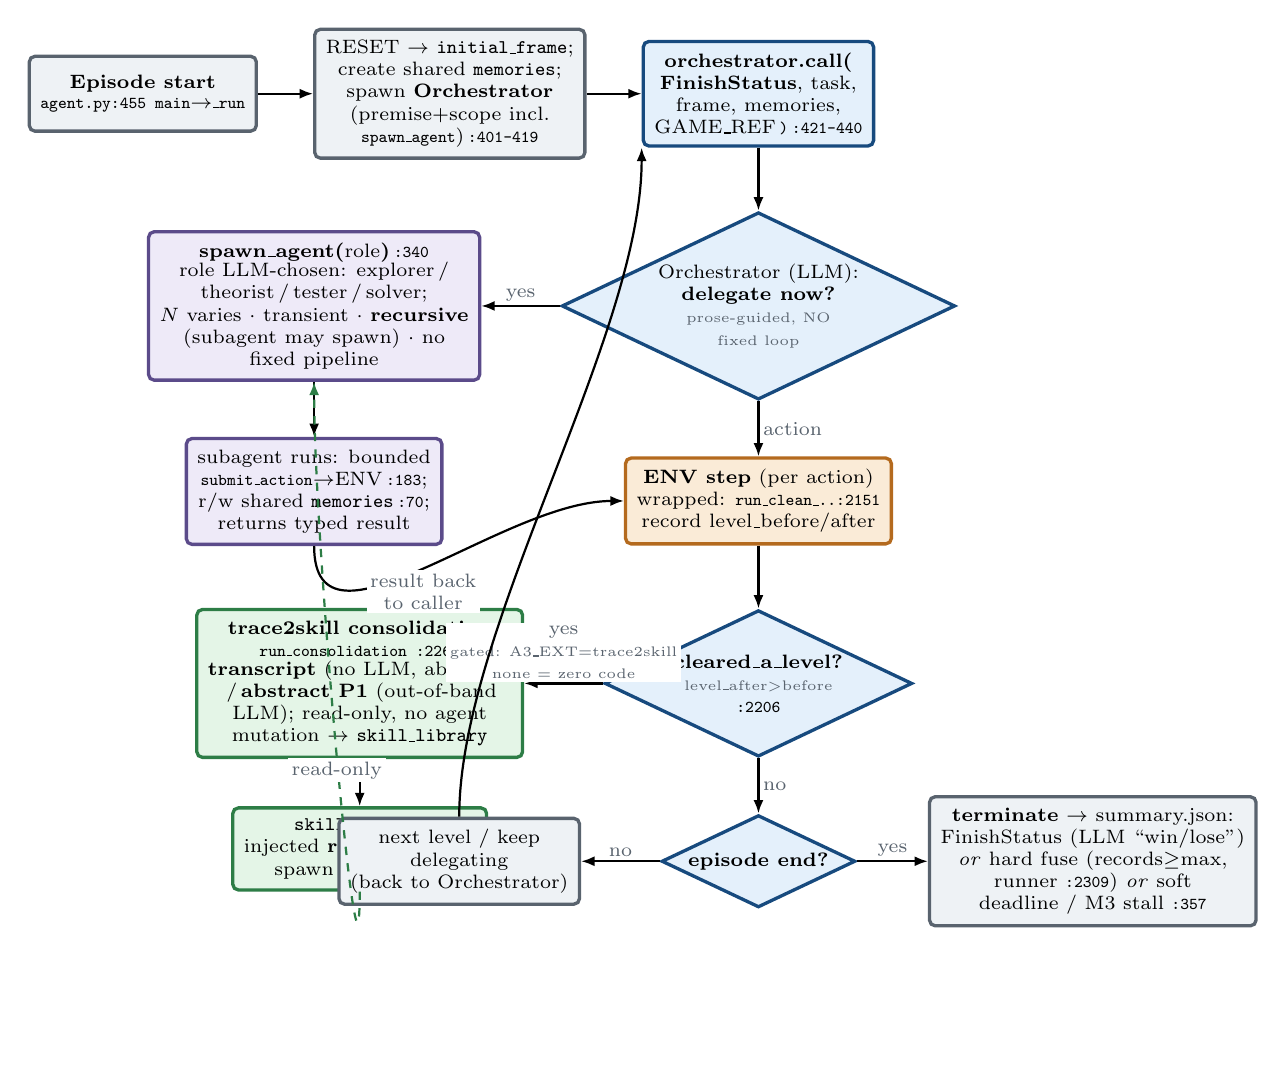
\begin{tikzpicture}[node distance=4mm]
  \node[st] (start) {\textbf{Episode start}\\[-1pt]\co{agent.py:455 main}$\to$\co{\_run}};
  \node[st, right=7mm of start] (init)
       {RESET $\to$ \texttt{initial\_frame};\\create shared \texttt{memories};\\
        spawn \textbf{Orchestrator}\\(premise+scope incl.\\\co{spawn\_agent})\,\co{:401-419}};
  \node[orc, right=7mm of init] (call)
       {\textbf{orchestrator.call(}\\\textbf{FinishStatus}, task,\\frame, memories,\\GAME\_REF\,\co{)}\,\co{:421-440}};

  \node[dec, below=8mm of call] (d1)
       {Orchestrator (LLM):\\\textbf{delegate now?}\\\fl{prose-guided, NO}\\\fl{fixed loop}};
  \node[sub, left=10mm of d1] (spawn)
       {\textbf{spawn\_agent(}role\textbf{)}\,\co{:340}\\[-1pt]role LLM-chosen: explorer\,/\\theorist\,/\,tester\,/\,solver;\\
        $N$ varies $\cdot$ transient $\cdot$ \textbf{recursive}\\(subagent may spawn) $\cdot$ no\\fixed pipeline};
  \node[sub, below=7mm of spawn] (act)
       {subagent runs: bounded\\\textbf{\co{submit\_action}}$\to$ENV\,\co{:183};\\
        r/w shared \texttt{memories}\,\co{:70};\\returns typed result};
  \node[env, below=7mm of d1] (envh)
       {\textbf{ENV step} (per action)\\wrapped: \co{run\_clean\_..:2151}\\
        record level\_before/after};

  \node[dec, below=8mm of envh] (d2)
       {\textbf{cleared\_a\_level?}\\\fl{level\_after>before}\\\co{:2206}};
  \node[t2s, left=10mm of d2] (cons)
       {\textbf{trace2skill consolidation}\\\co{run\_consolidation :2269}\\[-1pt]
        \textbf{transcript} (no LLM, ablation)\\\,/\,\textbf{abstract P1} (out-of-band\\LLM); read-only, no agent\\mutation $\to$ \texttt{skill\_library}};
  \node[t2s, below=6mm of cons] (lib)
       {\texttt{skill\_library}\\injected \textbf{read-only} into\\spawn scope \co{:1371}};

  \node[dec, below=7mm of d2] (d3)
       {\textbf{episode end?}};
  \node[st, left=10mm of d3] (loop) {next level / keep\\delegating\\(back to Orchestrator)};
  \node[st, right=9mm of d3] (term)
       {\textbf{terminate} $\to$ summary.json:\\FinishStatus (LLM ``win/lose'')\\
        \emph{or} hard fuse (records$\ge$max,\\runner \co{:2309}) \emph{or} soft\\deadline / M3 stall \co{:357}};

  \draw[ar] (start) -- (init);
  \draw[ar] (init) -- (call);
  \draw[ar] (call) -- (d1);
  \draw[ar] (d1) -- node[el,above]{yes} (spawn);
  \draw[ar] (spawn) -- (act);
  \draw[ar] (act.south) to[out=-90,in=180] node[el,below,align=center]
       {result back\\to caller} (envh.west);
  \draw[ar] (d1) -- node[el,right]{action} (envh);
  \draw[ar] (envh) -- (d2);
  \draw[ar] (d2) -- node[el,above,align=center]
       {yes\\\fl{gated: A3\_EXT=trace2skill}\\\fl{none $=$ zero code}} (cons);
  \draw[ar] (cons) -- (lib);
  \draw[ar, draw=GreenA, dashed] (lib.south) to[out=-90,in=-90,looseness=0.8]
       node[el,below]{read-only} (spawn.south);
  \draw[ar] (d2) -- node[el,right]{no} (d3);
  \draw[ar] (d3) -- node[el,above]{no} (loop);
  \draw[ar] (loop.north) to[out=90,in=-90,looseness=0.7] (call.south west);
  \draw[ar] (d3) -- node[el,above]{yes} (term);
\end{tikzpicture}}

\vspace{0.4em}
{\footnotesize \textbf{Key:} \texttt{spawn\_agent} is a \emph{callable in the
orchestrator's scope} --- the LLM decides \emph{whether/when} to spawn (no
forced loop, $N$ dynamic, subagents transient \& recursive). trace2skill fires
\emph{only} on a level-clear \emph{and only} under \co{A3\_EXT=trace2skill}
(\co{none} runs zero of it); consolidation never mutates the agent
(read-only). Runner owns hard termination at the per-action chokepoint.}
\end{frame}
\end{document}
